\chapter{Convertisseur}

Convertisseur is a Python-based script that prepares input files for 'extended source' block of 'input.spec' file of SEM3D code. The input files are in hdf5 format and includes certain attributes. Two different scripts are provided for the cases where input motion is inserted by force-time history (force option) or moment-time history (moment option). \\


First, for 'moment' option, 'convert\textunderscore extended\textunderscore MOMENT.py' file is referred to. The file is self-explanatory and input data are defined between the lines 31-72 of the file, Figure \ref{con1}. \\


%% FIGURE : convert_moment
\begin{center}
\leavevmode
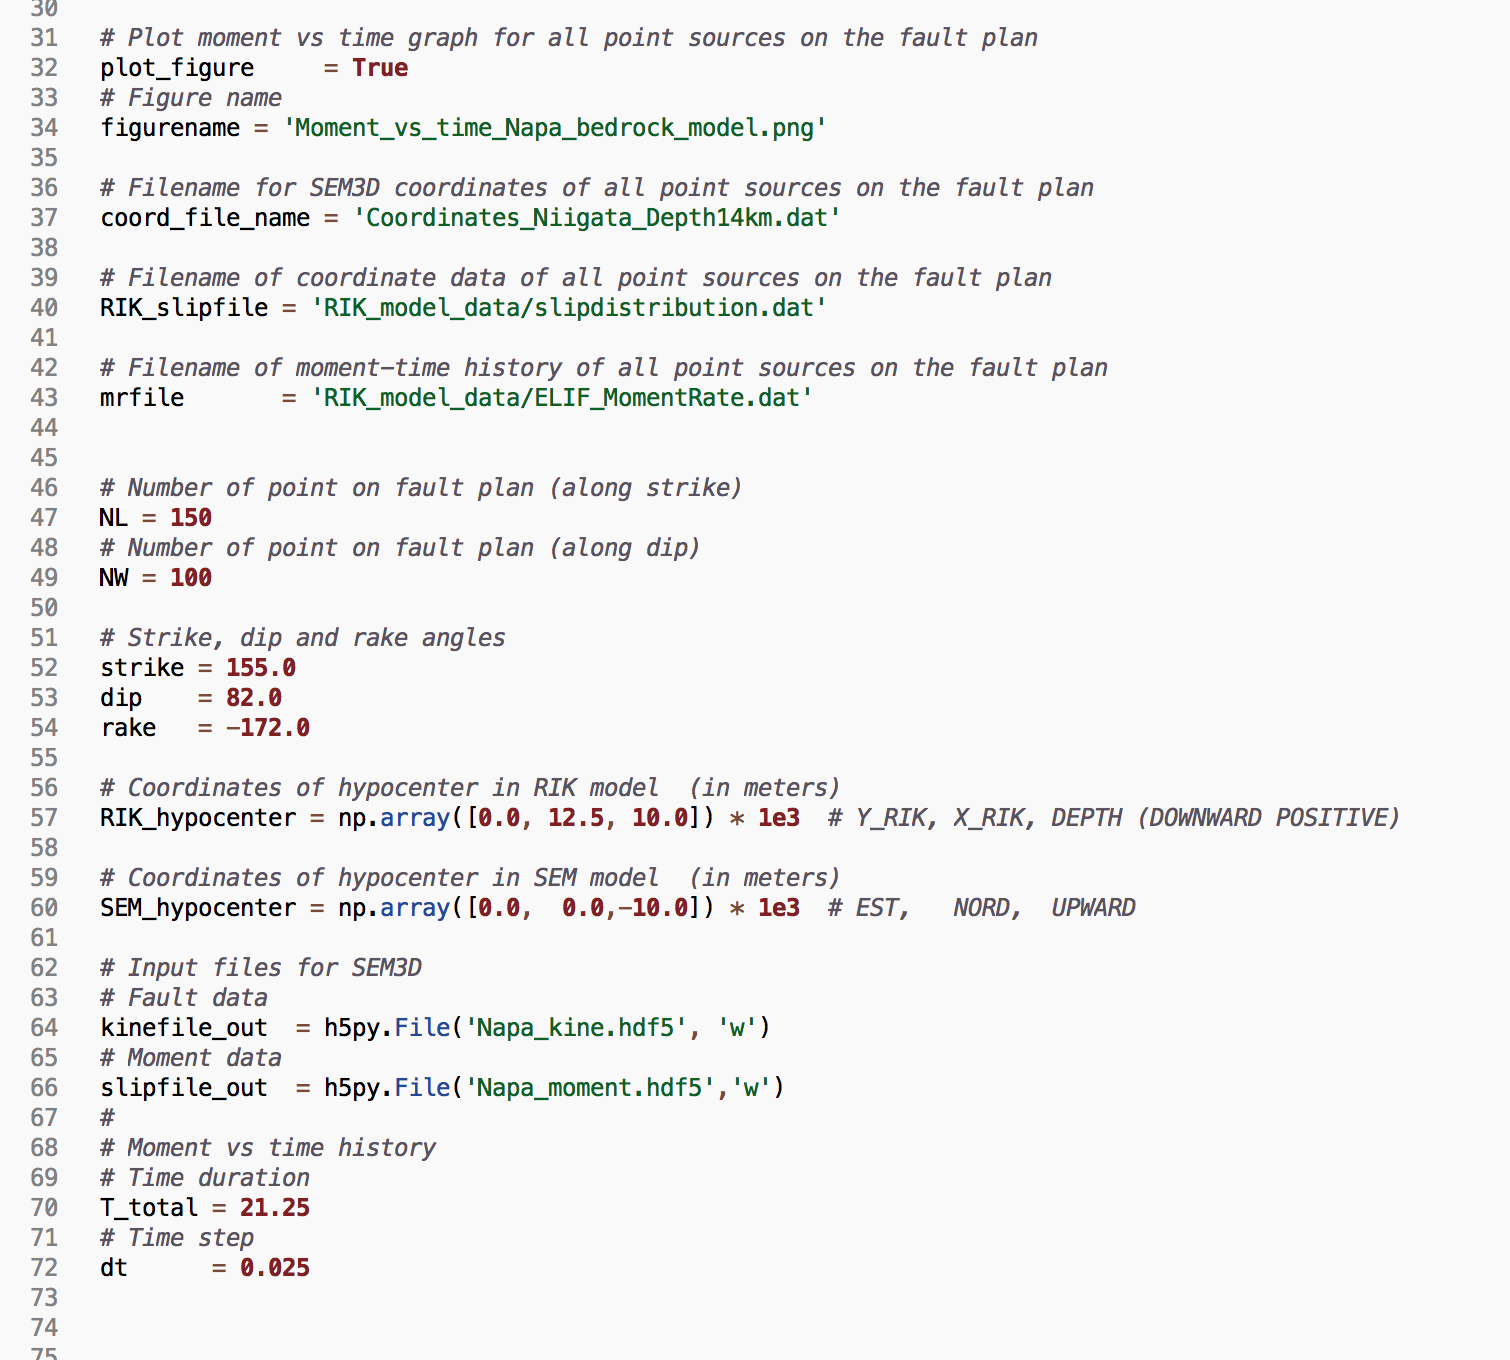
\includegraphics[scale=0.45]{figures/convert-moment.png} 
\captionof{figure}{The section with user data from convert\textunderscore extended\textunderscore MOMENT.py file for Napa example.}
\label{con1} 
\vspace{1cm}
\end{center}


In lines 31-34, the user should specify whether saving the figure of moment-time history of all the source points is desired or not. \\

In line 37, the name of file where the coordinates of the source points based on SEM3D model are written out is determined. \\

In line 40, the 'slipdistribution.dat' output file of RIK model (See Chapter \ref{chapRIK}) is defined. Coordinates of each point in RIK fault plan is read by this file. Similarly, in line 43, 'ELIF\textunderscore MomentRate.dat' file is defined to read moment-rate time history at each source point. The user could modify this part of the code if further modifications are desired concerning the employment of different source models. \\


In lines 47-49, number of points along strike and dip (the same as what is used in RIK model) are given. \\

In lines 52-54, strike, dip and rake angles are specified.  \\

In line 57, the hypocenter location of RIK model is written. It should be noted that the first term is the y-coordinate for RIK model, wherease the second term is the x-coordinate. In line 60, hypocenter location in SEM coordinates are written. \\

In lines 64-66, the names of files where fault properties and moment-time histories are to be written out are defined with hdf5 extension. \\


Lastly, in lines 70-72, time step and total duration used for moment-time histories are given. \\
 


Once the code is executed, it writes out following attributes in 'kinefile\textunderscore out' file:

\begin{itemize}
\item 'Ns'      : number of points along strike \\
\item 'Nd'      : number of points along dip    \\
\item 'Vnormal' : normal vector \\
\item 'Vslip'   : slip vector   \\
\item 'x'       : x-coordinates (SEM3D) of point sources \\
\item 'y'       : y-coordinates (SEM3D) of point sources \\
\item 'z'       : z-coordinates (SEM3D) of point sources \\
\end{itemize}



Slip vector is computed by the formula: \\

\begin{equation}
$$ \[
V_{slip}=
  \begin{bmatrix}
    sin\lambda cos\delta cos\phi + cos\lambda sin\phi     \\
    sin\lambda cos\delta sin\phi + cos\lambda cos\phi     \\
    sin\lambda sin\delta             				     \\
  \end{bmatrix}
\]
$$
\end{equation}

where $\phi$ holds for strike angle and $\delta$ corresponds to dip angle and $\lambda$ is rake angle of the fault plan. \\


For the computation of normal vector, we refer to the following formula: \\

\begin{equation}
$$ \[
V_{normal}=
  \begin{bmatrix}
    sin\delta cos\phi    \\
   -sin\delta sin\phi    \\
    cos\delta		     \\
  \end{bmatrix}
\]
$$
\end{equation}




The SEM3D coordinates are calculated by rotation and translation. Rotation is applied by multiplication of coordinate vector with rotation matrix. The rotation matrix is shown below: \\


\begin{equation}
$$ \[
R=
  \begin{bmatrix}
    -cos\phi cos\delta  & sin\phi  & 0 \\
     sin\phi cos\delta  & cos\phi  & 0 \\
     0 				    & 0 		  & -1
  \end{bmatrix}
\]
$$
\end{equation}




Following the rotation, translation is applied based on the difference between hypocenter points of RIK and SEM coordinates systems. \\


By means of provided data, the code integrates the given moment-rate histories to calculate moment-time histories. In the 'slipfile\textunderscore out' file, calculated moment and time data are prepared as follows:
\begin{itemize}
\item 'moment'    : moment history for point sources \\
\item 'time'      : time history for point sources    \\
\end{itemize}



The resultant moment-time history for 15000 point sources in this example is shown in Figure \ref{momo} .

%% FIGURE : convert_moment
\begin{center}
\leavevmode
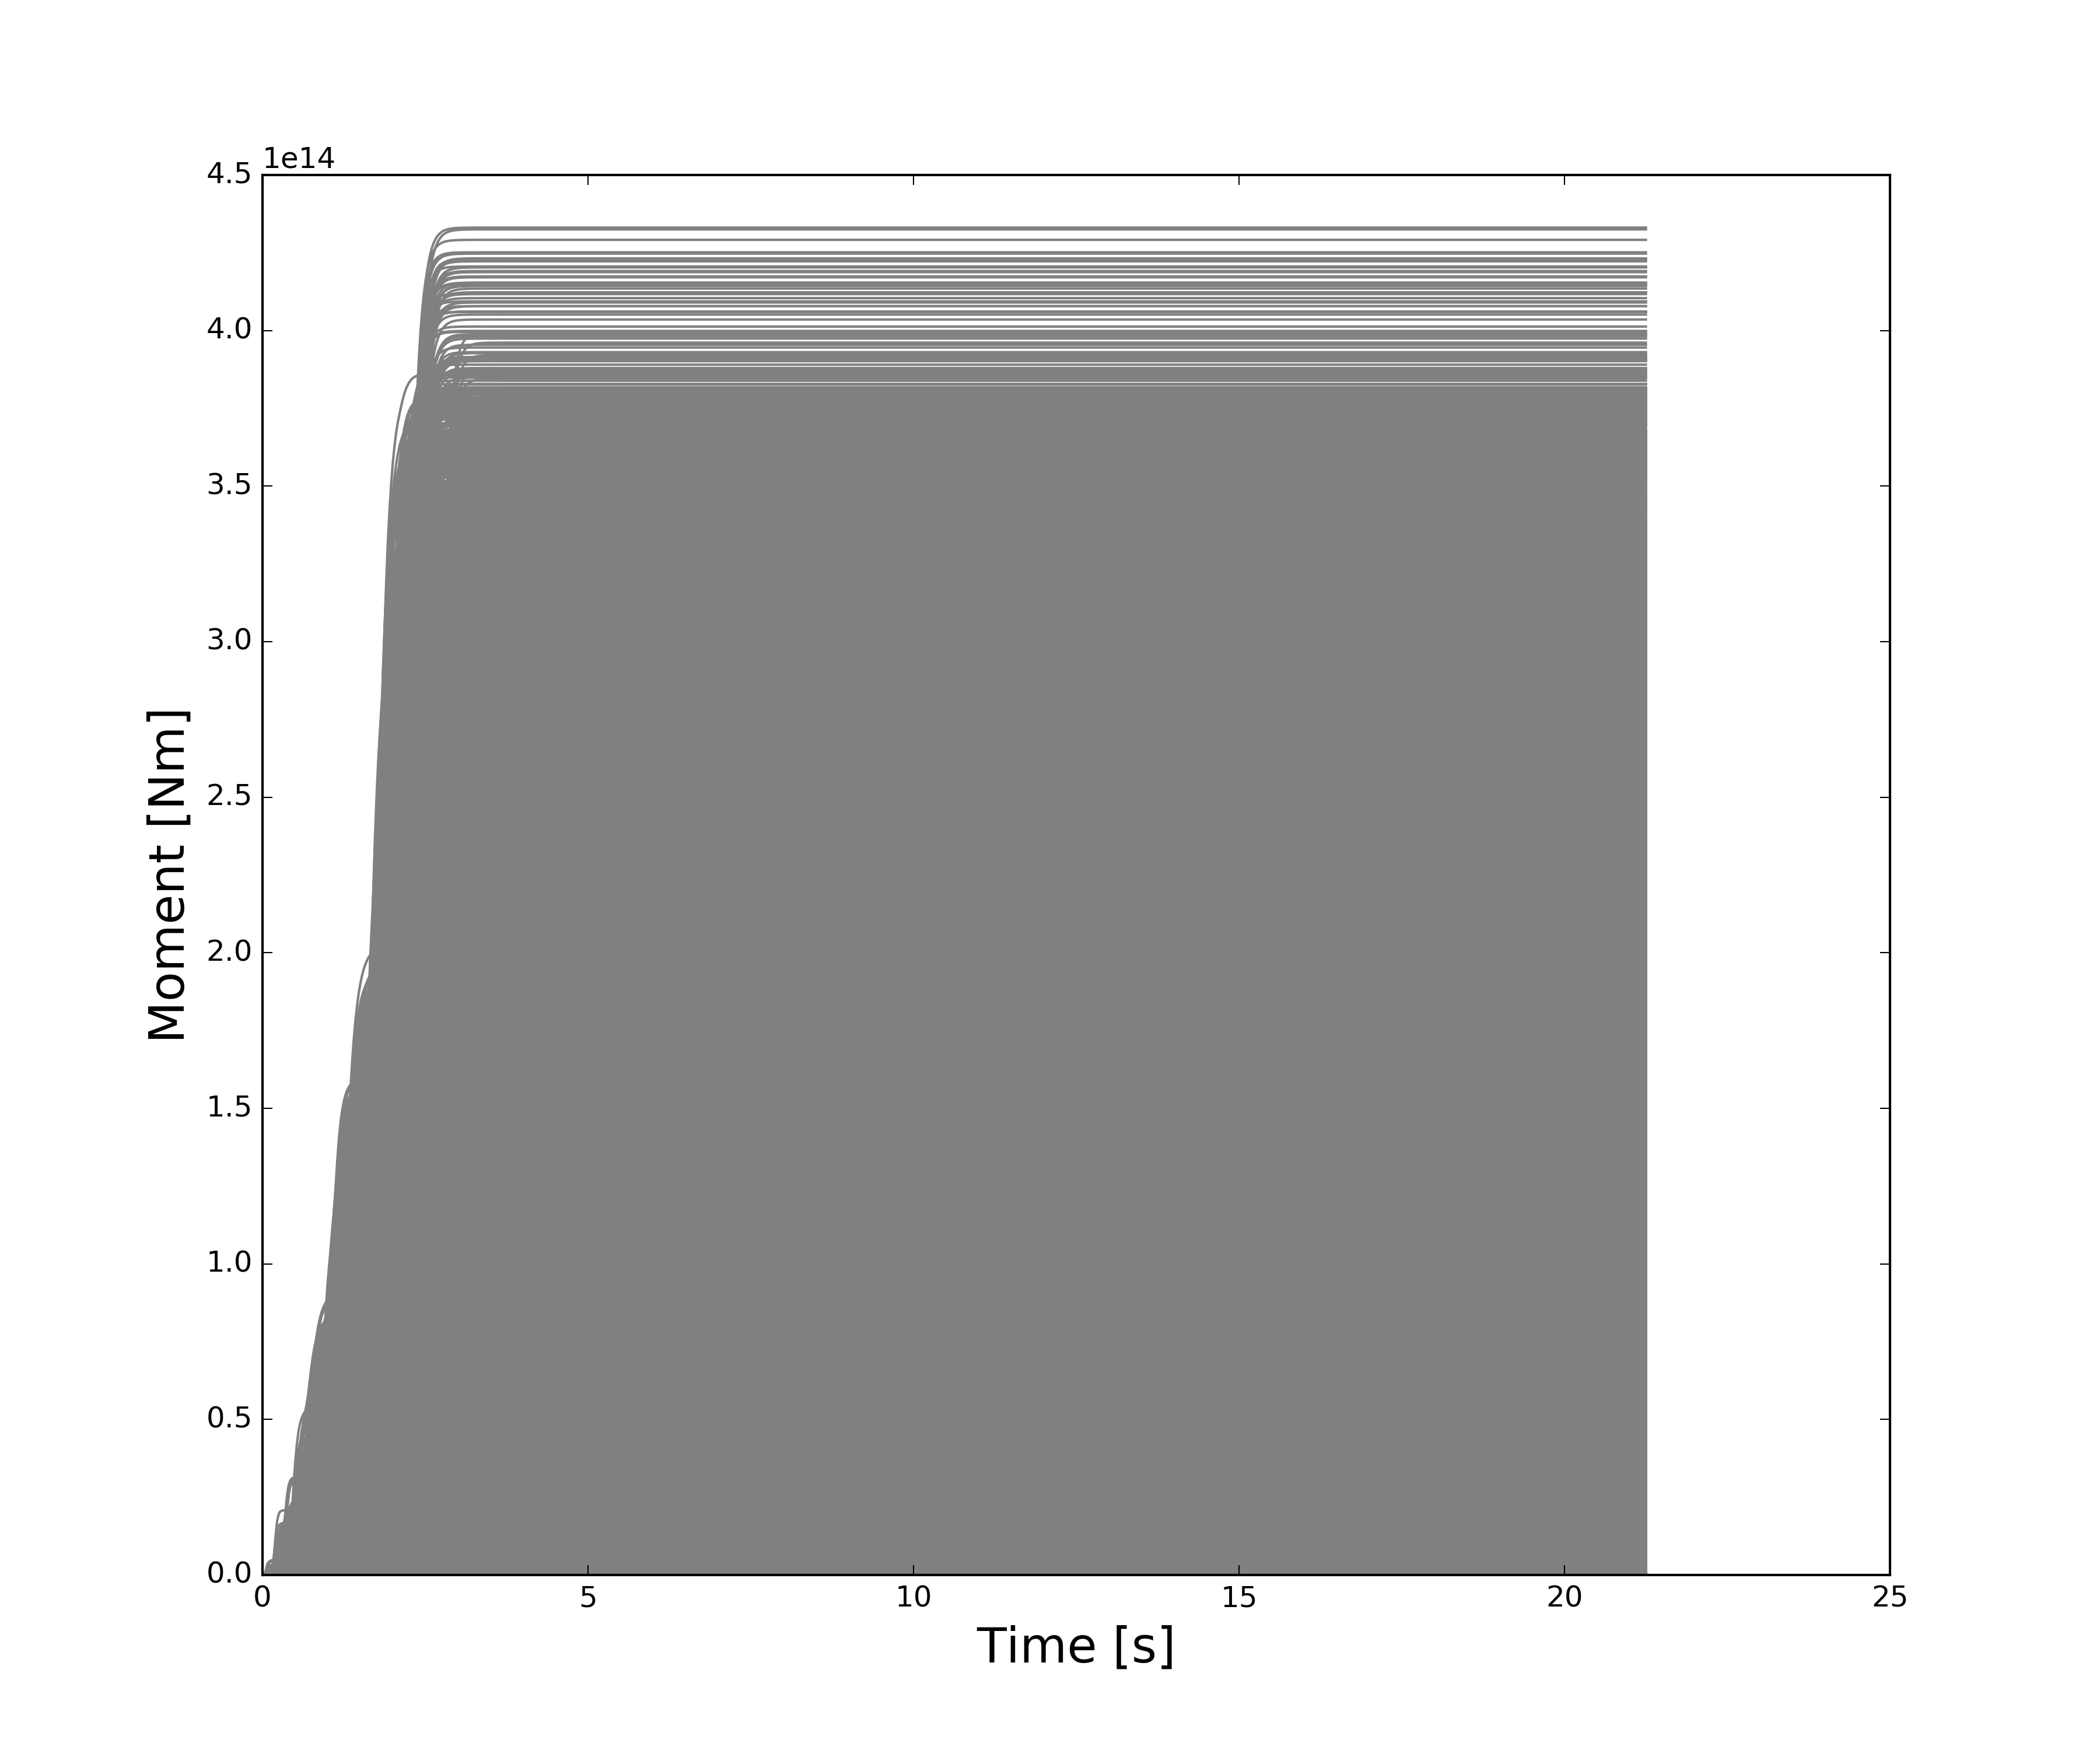
\includegraphics[scale=0.45]{figures/Moment_vs_time_Napa_bedrock_model.png} 
\captionof{figure}{Moment-time history of source points on extended fault plan for Napa example.}
\label{momo} 
\vspace{1cm}
\end{center}






%%% FORCE %%%
 
As a second option, 'convert\textunderscore extended\textunderscore FORCE.py' file could be referred to for cases where the source is defined by force-time histories. The file is self-explanatory and input data are defined between the lines 26-76 of the file, Figure \ref{con2}. As an example, we use three point sources of which force-time histories are defined by DM function. \\


%% FIGURE : convert_moment
\begin{center}
\leavevmode
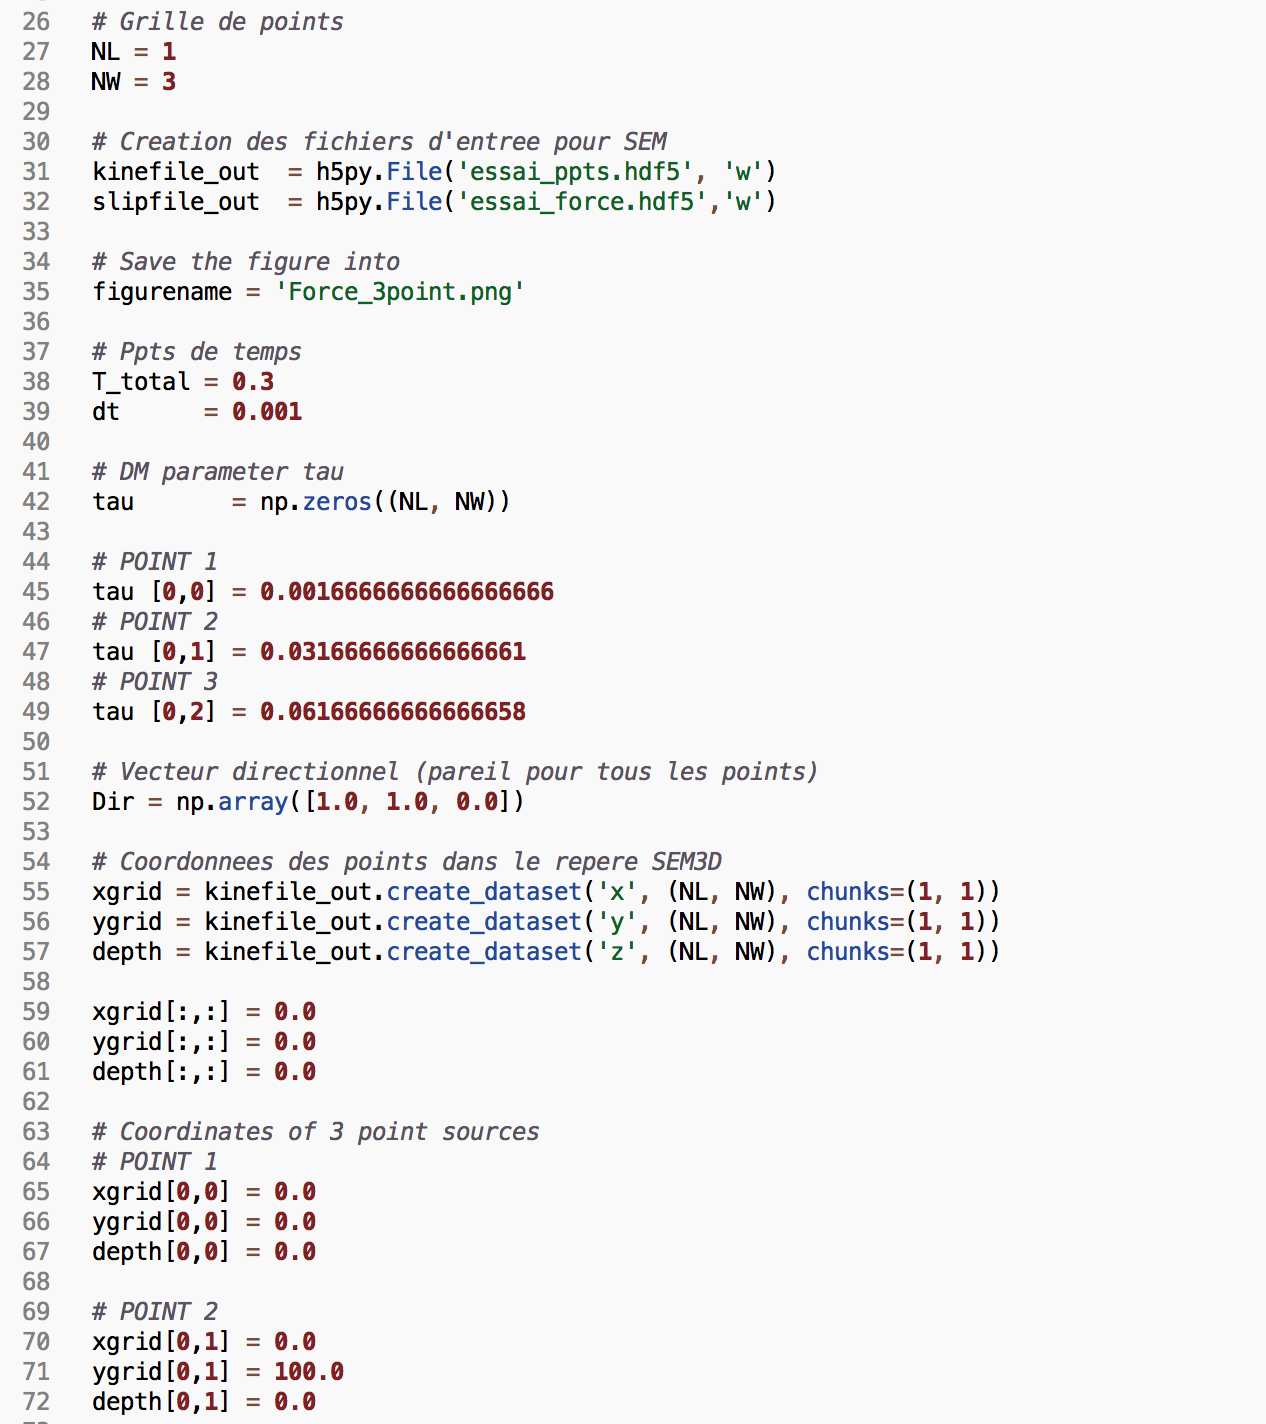
\includegraphics[scale=0.45]{figures/convert-force.png} 
\captionof{figure}{The section with user data from convert\textunderscore extended\textunderscore FORCE.py file for Napa example.}
\label{con2} 
\vspace{1cm}
\end{center}


Differently than moment option, here, we define $\tau$ parameter (time off-set) in DM function for each point source (Lines 45-49). Also, in line 52, direction vector is given and it is considered the same for all point sources. Lastly, x, y and z-coordinates of the point sources are defined. The resultant kinefile\textunderscore out comprises of following attributes: \\


\begin{itemize}
\item 'Ns'      : number of points along strike \\
\item 'Nd'      : number of points along dip    \\
\item 'Dir'     : direction vector \\

\item 'x'       : x-coordinates (SEM3D) of point sources \\
\item 'y'       : y-coordinates (SEM3D) of point sources \\
\item 'z'       : z-coordinates (SEM3D) of point sources \\
\end{itemize}


To save force-time function, the code uses following attributes:\\
\begin{itemize}
\item 'moment'    : force history for point sources \\
\item 'time'      : time history for point sources    \\
\end{itemize}



We show the resultant force-time histories for the three point sources in this example, Figure \ref{fofo}. \\


% FIGURE : convert_moment
\begin{center}
\leavevmode
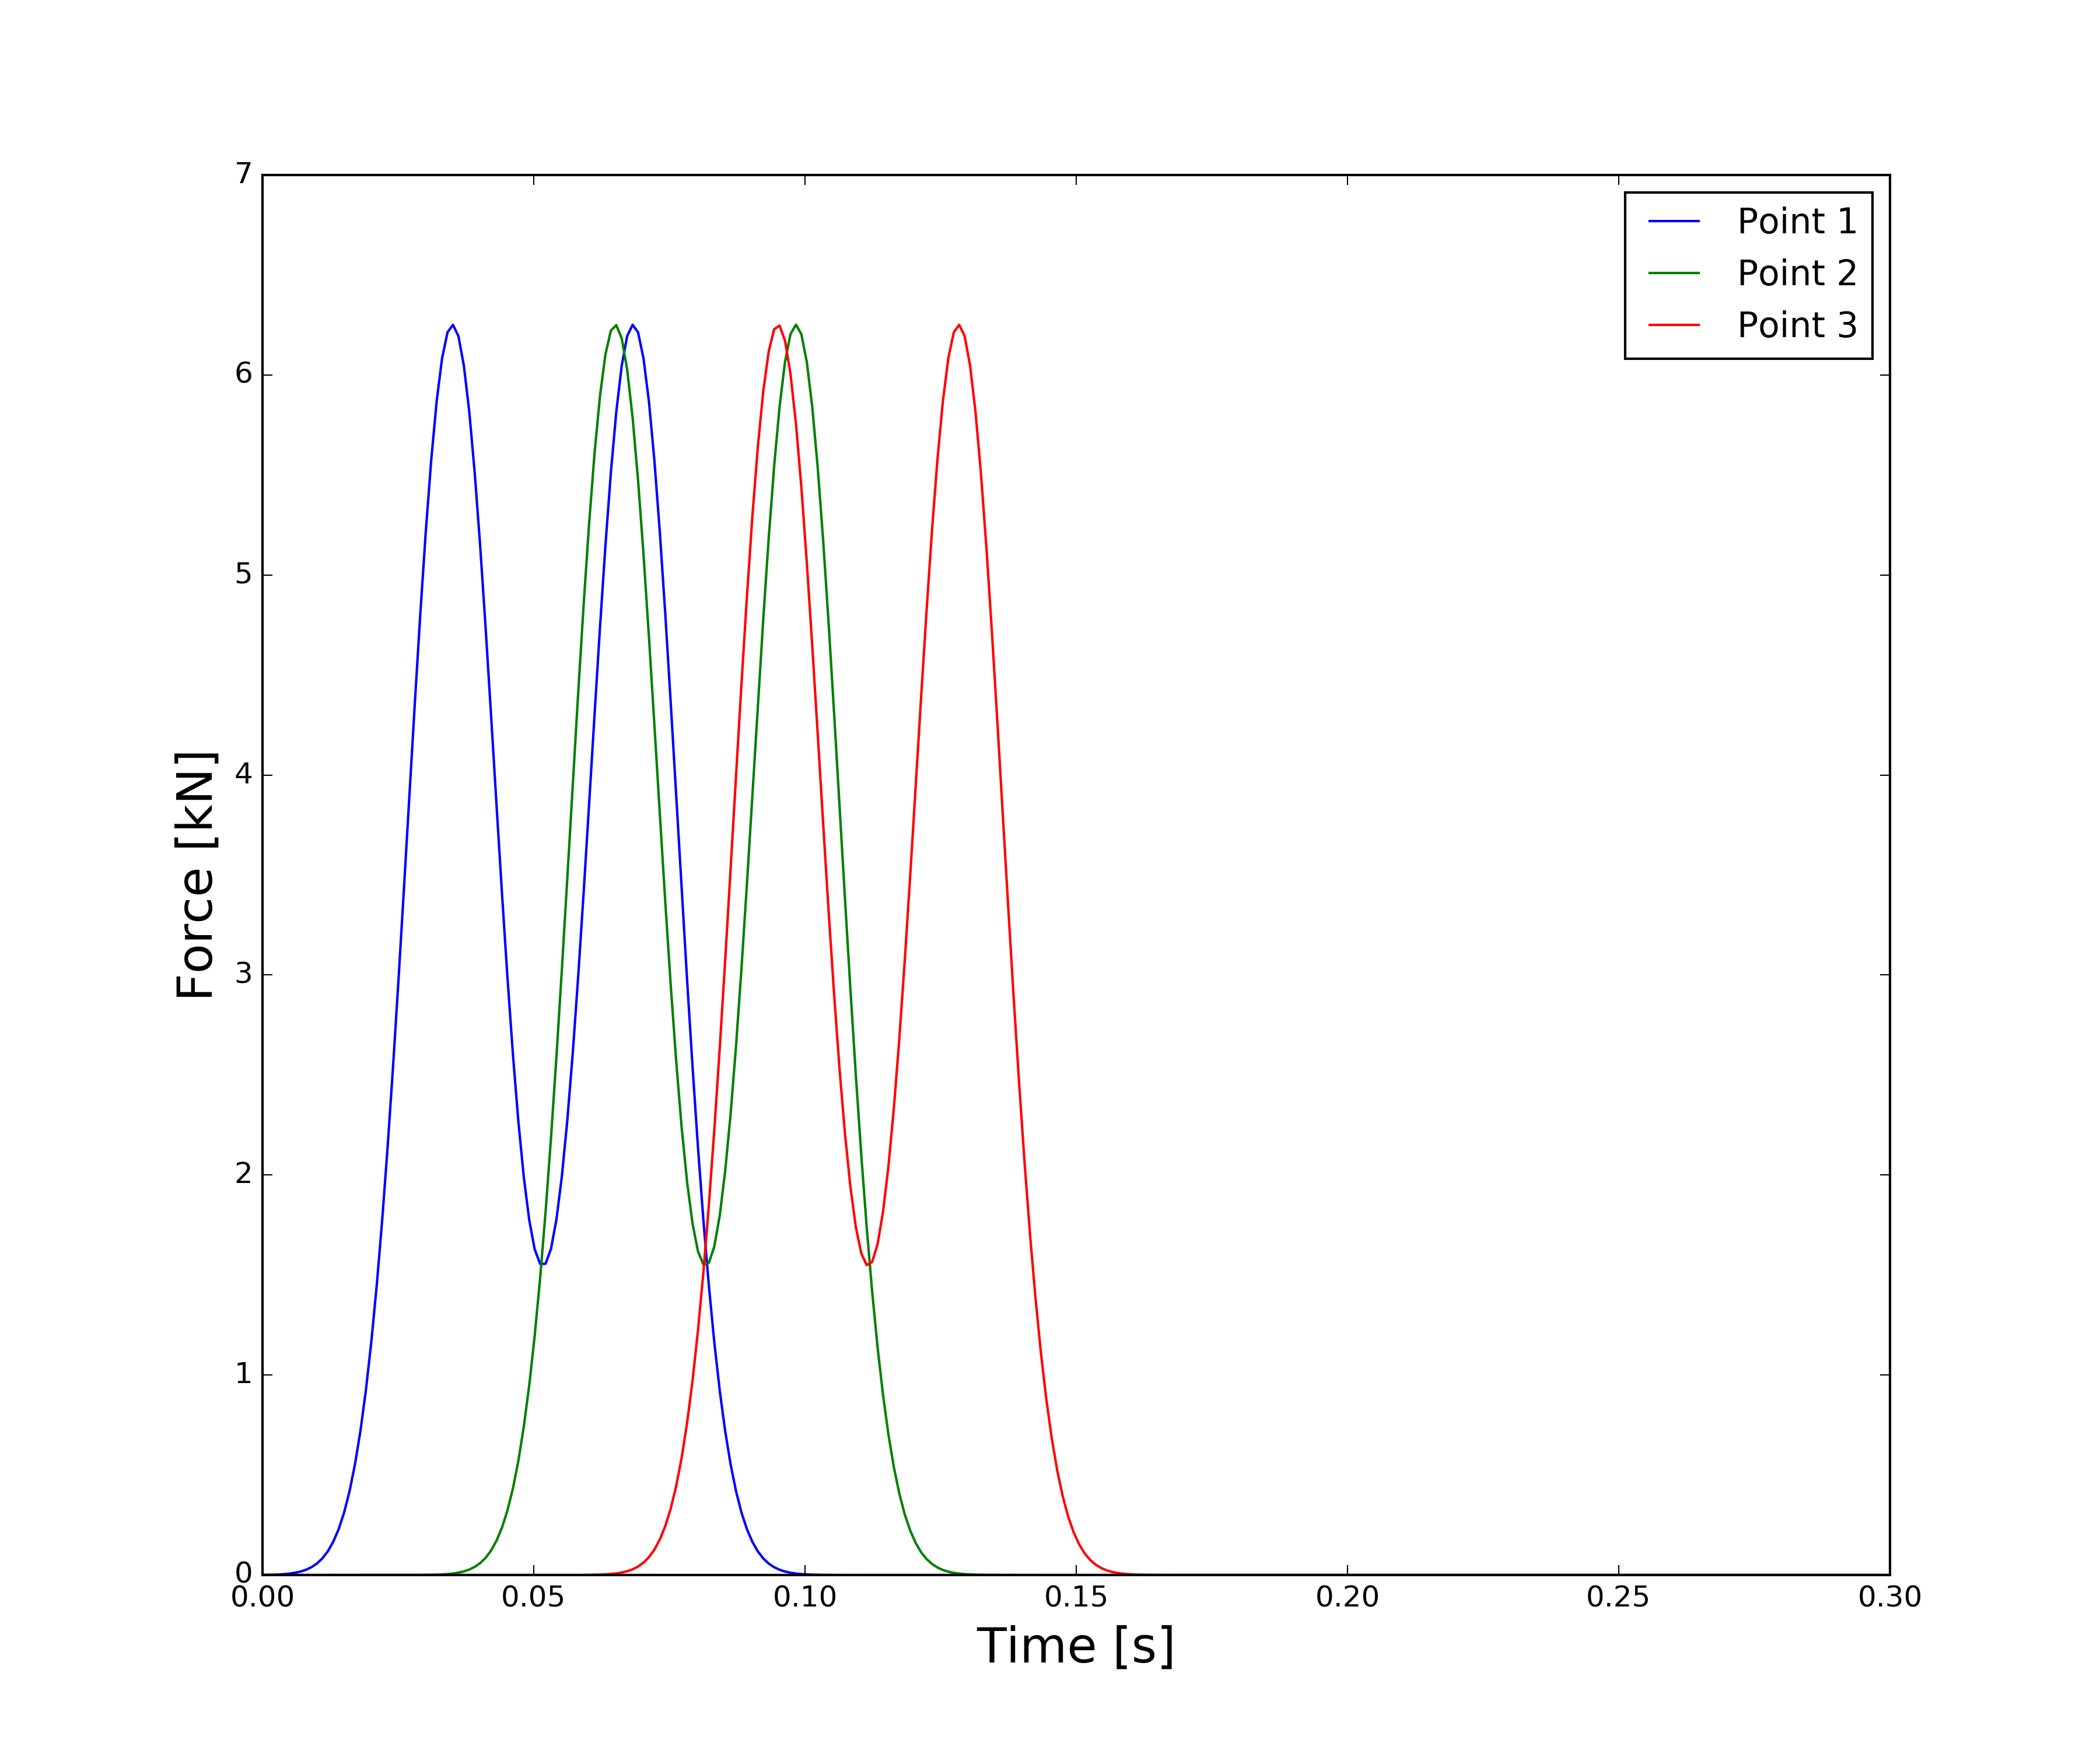
\includegraphics[scale=0.45]{figures/Force_3point.png} 
\captionof{figure}{Force-time history of the three source points.}
\label{fofo} 
\vspace{1cm}
\end{center}






















 